% $Id: preview.tex,v 1.19 1998/06/22 08:07:00 ohl Exp $
%%%%%%%%%%%%%%%%%%%%%%%%%%%%%%%%%%%%%%%%%%%%%%%%%%%%%%%%%%%%%%%%%%%%%%%%


\NeedsTeXFormat{LaTeX2e}
\documentclass[11pt]{article}
\usepackage{amsmath,amssymb,amsthm}
\usepackage[margin=1.0in]{geometry}
\usepackage{amscd}
\usepackage{epsfig}
\allowdisplaybreaks
\setlength{\unitlength}{1mm}
%%%%%%%%%%%%%%%%%%%%%%%%%%%%%%%%%%%%%%%%%%%%%%%%%%%%%%%%%%%%%%%%%%%%%%%%
\makeindex
\begin{document}
\title{\bf {PURE DATA SPACES....DRAFT...DRAFT...DRAFT}}
\author{%
  SAUL YOUSSEF%
  \hfil \\
  Department of Physics \\
  Boston University \\
}
\maketitle
\begin{abstract}
All about spaces.
\end{abstract}
%%%%%%%%%%%%%%%%%%%%%%%%%%%%%%%%%%%%%%%%%%%%%%%%%%%%%%%%%%%%%%%%%%%%%%%%

%%%%%%%%%%%%%%%%%%%%%%%%%%%%%%%%%%%%%%%%%%%%%%%%%%%%%%%%%%%%%%%%%%%%%%%%

\newtheorem*{fact}{Fact}

\newtheorem{definition}{Definition}

\newtheorem*{remark}{}

\section{Overview}

In Reference 1, we introduced a tiny axiomatic framework, based on the {\bf finite sequence} as a foundational concept.  
With finite sequences understood, we had 
\begin{itemize}
\item[1 ]{\it ``Data" is a finite sequence of ``codas,'' where each coda is a pair of data.}
\end{itemize}
\noindent This kind of data, such as (:)\ (:(:))\ ((:):(:)\ (:)), is ``pure data'' in the sense that it is ''made of nothing.'' Such data has two natural operations: 
{\it concatenation} of data A with data B, written (A\ B), and {\it pairing} data A and data B as a {\it coda}, written (A:B).  
\begin{itemize}
\item[2 ]{\it Definitions are embodied by a chosen partial function $\delta$ from codas to data called a context.}
\end{itemize}
As modest as it is, 1 and 2 appear to be able to capture Mathematics in general.  Consequences include:   
\begin{itemize}
\item[-]{Fixed points of $\delta$ ({\it atoms}), represent fixed data such as bits, bytes and text;}
\item[-]{Data outside the domain of $\delta$ are {\it variables}, which might become defined over time as {\it definitions} are added to $\delta$;} 
\item[-]{$\delta$ contains it's own {\it language}, allowing user specification of data and adding definitions to $\delta$;} 
\item[-]{Equality of data A=B is determined by $c\sim\delta(c)$ and by compatibility with finite sequences. Proof and computation are then defined by the equality.  A sequence $A_1=A_2=\dots=A_n$ is both a proof of $A_n$ given $A_1$ and a computation $A_1\mapsto A_n$.  Proof and computation are essentially the same thing;}
\item[-]{Data is {\it true} if it is empty, {\it false} if it is atomic, and {\it undecided} otherwise.  Undecided data may also be {\it undecidable}, as in the Godel phenomena or other seeming paradoxes.  Data which is {\it never false} as definitions are added is a {\it theorem}.}
\end{itemize}

In this work, we investigate the concept of a {\it space}, introduced in Reference 1.  

\begin{figure}[h]
\centering
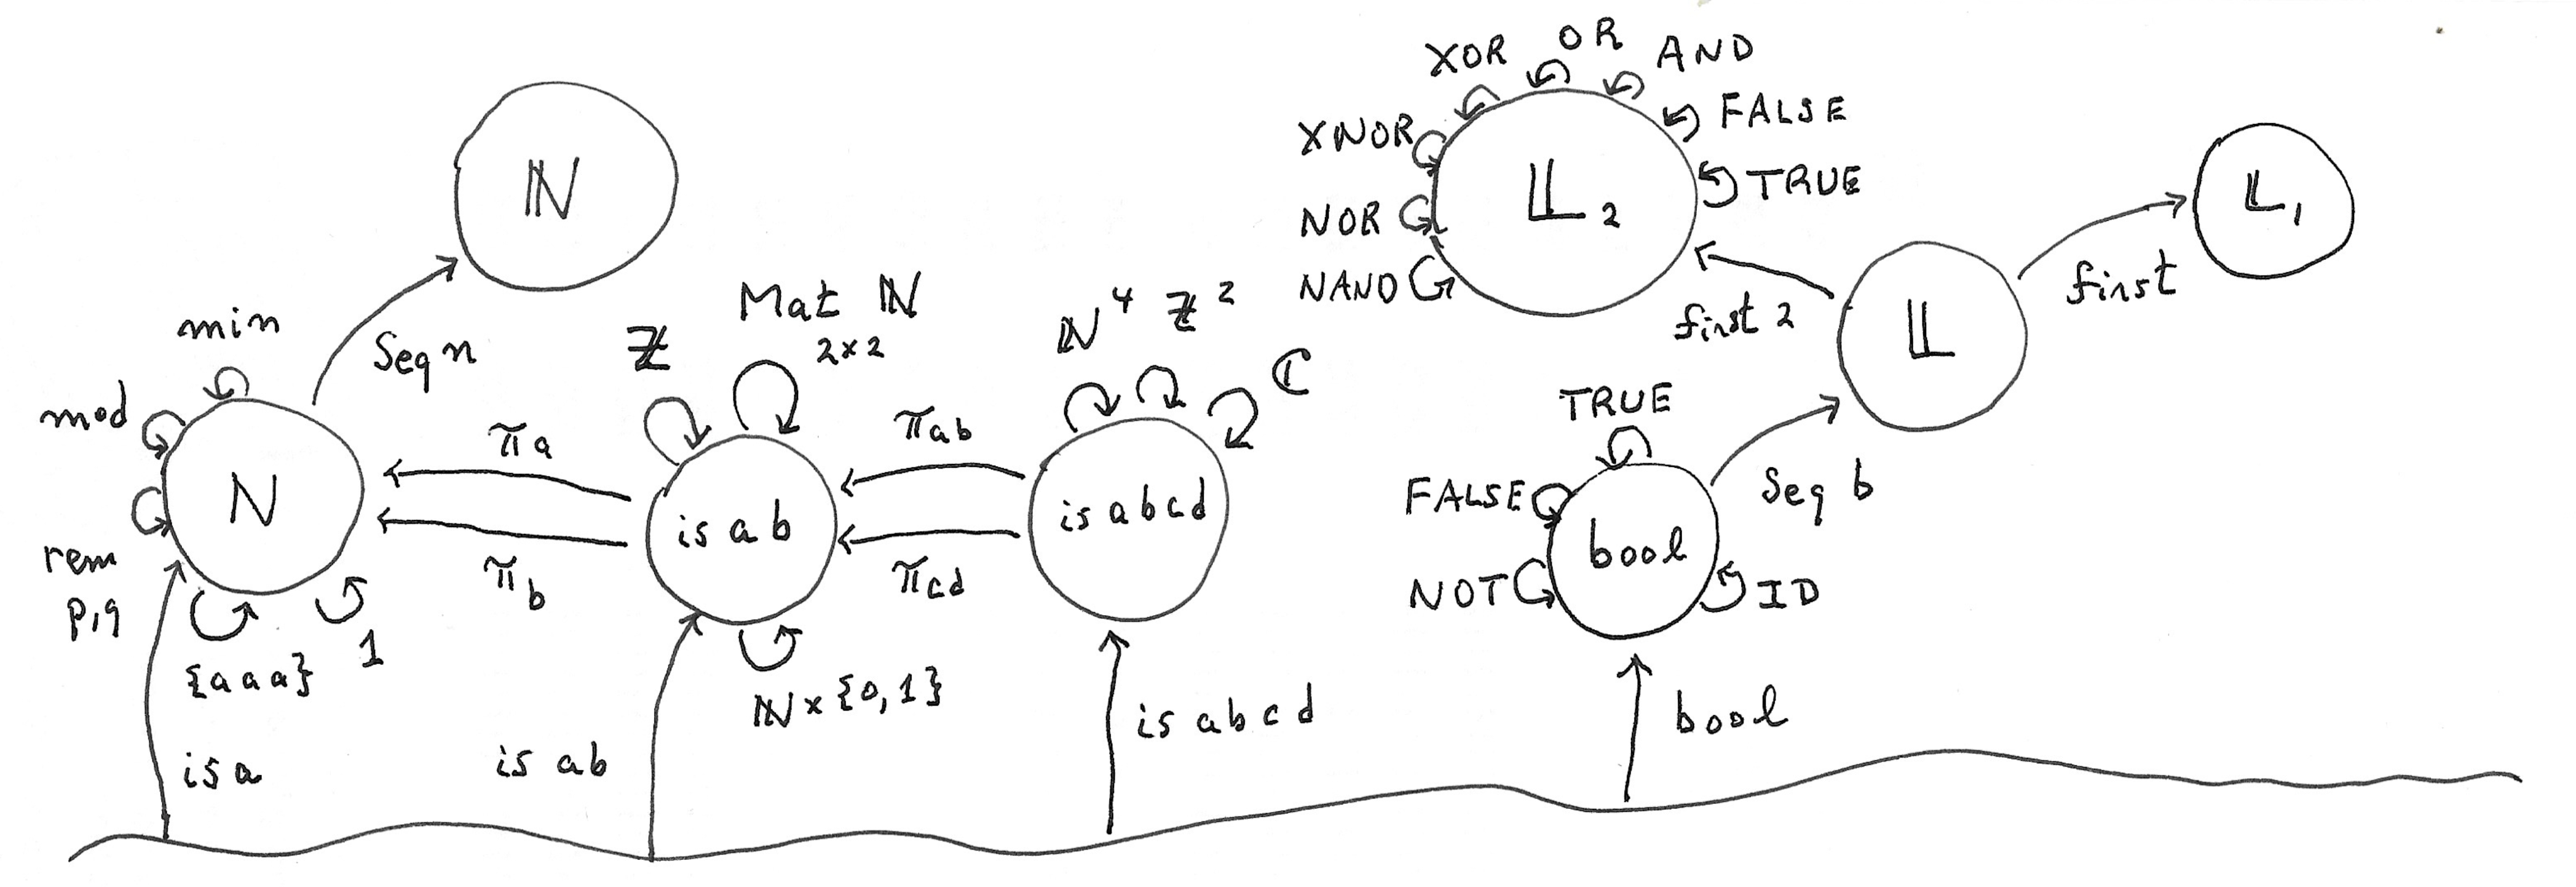
\includegraphics[width=0.7\textwidth]{garden.png}
\caption{{\it Growing spaces ``organically'' from pure data.}}
\end{figure}


...SEARCHING....ORGANICS....

\section{Foundation}  

In \cite{PDF}, we argue that Mathematics and Computing as a whole can be captured within a tiny framework, based only on {\bf finite sequence} as the foundational undefined concept.  Assuming that finite sequences are understood, we define {\it data} and {\it coda} as follows.   

\begin{definition} {Data is a finite sequence of {\bf codas}, where each {\bf coda} is a pair of {\bf data}.}
\end{definition}

\noindent Concatenation of data A and data B as finite sequences is denoted by ``A\ B" and the pairing of data A and data B as a coda is written as ``A:B" with a colon indicating 
the pairing from the definition.  
By the definition, the empty sequence ``written ()" qualifies as data and, therefore, () paired with itself is a coda (written ``(:)").  Any finite sequence of codas is data, so, for example (:)\ (:(:))\ ((:):(:(:))) is  
data consisting of a sequence of three codas.  We call this {\it pure data} because it is {\it data made of nothing.}  By convention, the colon binds from the right first and binds less strongly than concatenation, so that A:B:C is defined to mean (A:(B:C)) and A:B\ C is defined to mean (A:(B\ C)).  Data is typically written with upper case, and codas are typically written in lower case.  To indicate the left and right data of a coda, we sometimes use L/R superscripts so that $c=(c^L:c^R)$. 

     All meaning within the system is determined by a single chosen partial function from coda to data called a {\bf context}. 
Contexts are partially ordered by inclusion, so if $\delta$ and $\delta'$ are contexts, $\delta\le\delta'$ if $\delta$ and $\delta'$ are equal on the domain of $\delta$.  
Given a context $\delta$, equality of data is determined by $c\sim \delta(c)$ for any coda $c$, and by compatibility with concatenation and colon: if A$\sim$B, then (A\ X)$\sim$(B\ X), (X\ A)$\sim$(X\ B), (A:X)$\sim$(B:X) and (X:A)$\sim$(X:B) for any data X.
Thus, if A${\overset \delta =}$B and $\delta\leq\delta'$, then A${\overset {\delta'} =}$B.  We may say that if A and B are equal then they are {\it always equal}, thinking of $\delta\rightarrow\delta'$ as the passage of time.  Note that any fixed point c of $\delta$ is stable in the sense that any ``later'' $\delta'$ must be identical to $\delta$ on c.  The fixed points of a given context $\delta$ are called {\it atoms}.  

\begin{definition}
{Within a given context $\delta$, coda $c$ is an {\bf atom} if $\delta:c\mapsto c$.  If data A contains an atom, A is {\bf atomic} data. 
Data A is {\bf invariant} if every coda $a$ in the sequence of $A$ is an atom and if $a^L$ and $a^R$ are both {\bf invariant}. }
\end{definition}
\noindent Note that empty data is invariant.  If $a$ and $b$ are atoms in context $\delta$ and if A and B are data, we have: 
1) $a$ and $b$ remain atoms in any context greater than or equal to $\delta$; 2) $a=b$ if and only if $a^L=b^L$ and $a^R=b^R$; 3) If ($a$\ A)=($b$\ B), then $a=b$ and A=B; 
4) If (A\ $a$)=(B\ $b$), then A=B and $a=b$; 5) If A and B are invariant and equal, then A and B are identical as pure data. 

Given a context $\delta$, we may write the corresponding equality as ${\overset \delta =}$ or, when not ambiguous, as $=$. 
If data A and B satisfy A:X${\overset \delta =}$B:X for all X, this equivalence is also often written simply as ``=" if is clear in context, as in the following definitions. 

\begin{definition}
Data A is 
\begin{itemize}
\item[-]{a {\bf constant} if (A:X) = (A:) for all X};
\item[-]{{\bf idempotent} if (A:A:X) = (A:X) for all X}; 
\item[-]{an {\bf involution} if (A:A:X) = X for all X}; 
\item[-]{{\bf commutative} if (A:X\ Y) = (A:Y\ X) for all X,Y}; 
\item[-]{{\bf distributive} if (A:X\ Y) = (A:X) (A:Y) for all X,Y};
\item[-]{{\bf associative} if (A:X\ Y) = (A:(A:X)\ Y) = (A:X\ (A:Y)) for all X,Y.}
\end{itemize}
\end{definition}
\noindent 
If one thinks of A:X\ Y as an A-specified product X${\overset A *}$Y, then associativity of A guarantees 
(X${\overset A *}$Y)${\overset A *}Z$ = X${\overset A *}$(Y${\overset A *}Z)$ for all X,Y,Z.  
It is also convenient to define a product and sum of data in general, corresponding to the two foundational finite sequence operations: concatenation and colon.
For data A and data B, let (A$\cdot$B):X = A:B:X and let (A$\oplus$B):X = (A:X)\ (B:X).  As binary operators on data, $\cdot$ and $\oplus$ are both associative, but 
neither is generally commutative. 

\section{Genesis}

    The mathematical objects that we are used to will all be represented as pure data, and all meaning about mathematical objects, including what constitutes a valid proof or a valid computation, is determined by an assumed context embodying a chosen collection of definitions.  For instance, a valid proof in $\delta$ is just a sequence 
A$_1{\overset \delta =}$ A$_2 {\overset \delta =} \dots {\overset \delta =} $A$_n$, 
 which can be viewed either as proving A$_1{\overset \delta =}$A$_n$ or as computing A$_1\mapsto$A$_n$.
This is discussed in \cite{PDF} and will gradually become clearer as we go.  The immediate issue is to understand what constitutes a ``valid'' definition and how to choose an initial context.     
    
     In the beginning, there are no definitions, and the corresponding context is uniquely the empty partial function from coda to data, $\delta_0$.
 Within $\delta_0$, data are equal only if they are identical as 
 pure data, the only valid proofs are $X{\overset \delta =}X$ for any $X$ and the only valid computations do nothing $X\mapsto X$ for any X. 
To define a non-empty context $\delta_0\le\delta$, we need a way to specify the domain of $\delta$ which is unchanged by any later  
later definition.  Since the empty sequence is the only invariant, the way to specify if a coda (A:B) is in the domain of $\delta$ is 
to require either A or B or both to be the empty sequence. In each of these cases, the coda (:) is within the domain of $\delta$, and so we must decide on what (:) maps to.  
There are three possibilities; 
\begin{enumerate}
\item{$\delta: (:) \mapsto ()$},
\item{$\delta: (:) \mapsto (:)$}, or 
\item{$\delta: (:) \mapsto \ anything\ other\ than\ ()\ or\ (:)$}. 
\end{enumerate}
Since pure data is {\it made of (:)}, choice 1 trivially causes all data to be equal to the empty sequence. On the other hand, choice 3 means that for any data A the number of (:) atoms in A grows without limit.  Choice 3 is degenerate in the sense that no computation could produce a final answer.  Thus, we are constrained to choice 2, meaning that (:) must be an atom in $\delta$ and, therefore, is an atom for any $\delta'\ge\delta$.  
It is convenient to generalize choice 2 and let $\delta:$(:X)$\mapsto$(:X) for all data X, so that every coda (:X) is an atom.

A context of the form 
\begin{equation}
	\delta_a: (a\ A:B) \mapsto \delta_a(A,B)
\end{equation}
for some invariant atom $a$ is called a {\bf definition}.  We conventionally restrict ourselves to 
contexts $\delta\cup\delta_a\cup\delta_b\cup\dots$ where $a$ is an invariant atom in $\delta$, $b$ is an invariant atom in $\delta\cup\delta_a$, $c$ is an invariant atom in $\delta\cup\delta_a\cup\delta_b$ and so forth.  By requiring $a$, $b$,\dots to be disjoint, we maintain the required context partial ordering.  If one thinks of our framework as an axiomatic system, the one axiom asserting that the empty context $\delta_0$ is {\it valid}, and any context greater than or equal to a valid context is also {\it valid}. 

\section{Spaces}

    Mathematics requires a way to make abstract collections of other mathematical objects.  Since data as defined is the only available material, the collection must 
``contain" data and the collection itself must be specified by some data, say S.  Given data S, there are a couple of plausible ways for S to define a collection.  
\begin{itemize}
\item[-]{The data in the collection is S:X for any data X;}
\item[-]{The data in the collection are the fixed points of S.}
\end{itemize}
These options can be made to coincide if we require S to be idempotent, so that S:X is always a fixed point.  For a collection S to be compatible with concatenation, we might expect that if S:X and S:Y are in the collection, then so is (S:X)\ (S:Y).  This is guaranteed if 
\begin{equation}
{\rm S : X\ Y = S : (S: X)\ (S:Y)}
\end{equation}
which follows if S is both idempotent and associative.  Thus we come to the concept of a {\it pure data space} or just {\it a space}.  
\begin{definition} Data S is a {\bf space} if S is idempotent and associative.
\end{definition}
\noindent Notice that idempotence guarantees compatibility with the colon and associativity guarantees compatibility with concatenation.  

The data (S:) is called the {\bf neutral data} of S.  
It is easy to check that idempotent distributive data is also associative and is thus also a space. 
Distributive spaces have the empty sequence as their neutral data [since (S:)=(S:()\ ())=(S:)\ (S:)=()].  A distributive space can be thought of as acting independently on each atom of ``input'' since if data 
X is a sequence x$_1$\ x$_2\dots$x$_n$ of atoms, S:X = (S:x$_1$) (S:x$_2$)$\dots$(S:x$_n$).  

\subsection{Plan} 

\subsection{Algebraic Data} 

\subsection{Growing Spaces Organically} 

\section{The theory of Spaces}

\subsection{Commuting spaces}
If spaces S and T commute, then S$\cdot$T is a space.  To see this, note that S commuting with T means that S$\cdot$T is idempotent, and for any data X and Y, 
(S$\cdot$T):X\ Y = S:T:X\ Y = S:T:(T:X)\ (T:Y) = T:S:(T:X)\ (T:Y) = S:T:(S:T:X)\ (S:T:Y) = (S$\cdot$T):((S$\cdot$T):X) ((S$\cdot$T):Y).

\subsection{Compatible Spaces}

We say that data A {\bf absorbs} data B if A$\cdot$B=A.  If A absorbs B and B absorbs A, we say that A and B are {\bf compatible}.  {\it Absorbs} is transitive in general, reflexive for idempotent data such as spaces, but is not symmetric.  Compatiblity, however, is an equivalence relation.  For examples:
\begin{itemize}
\item[-]{Idempotent data is compatible with itself.}
\item[-]{{\bf null} absorbs any data}.
\item[-]{Any data absorbs {\bf pass}}.
\item[-]{The constant spaces \{a\} and \{b\} are compatible, but are not equal.}
\end{itemize}
Any data that is compatible with a space is a space itself.  To prove this, let S be a space and A be any data where S$\cdot$A=S and A$\cdot$S=A.
Then A$\cdot$A=A$\cdot$S$\cdot$A$\cdot$S=A$\cdot$S=A, so A is idempotent, and A:X\ Y = (A$\cdot$S):X\ Y = A:S:(S:X)\ (S:Y) = A:S:(S:A:X)\ (S:A:Y) = A:S:(A:X)\ (A:Y) = 
A:(A:X)\ (A:Y), so A is a space. 

\subsection{Kernels, Positive Spaces, and Complementary Spaces}

Data X is {\bf in the kernel} of space S if (S:X)=(S:), and we denote this by X$\in $Ker(S).  For any space S, if X$\in $Ker(S) and Y$\in $Ker(S), then X\ Y$\in$Ker(S).  
If the converse is true, we say that $S$ is a {\bf positive} space.  Simple facts and examples follow.  
\begin{enumerate}
\item[-]{Every distributive space is positive, since if S:X\ Y=(S:)=(), so (S:X)\ (S:Y)=(), and, thus (S:X) and (S:Y) are both empty}.
\item[-]{However, not all positive spaces are distributive, for example, ({\bf front} $\vert\ \vert$) is a positive space, but not a distributive space}.
\item[-]{If S is positive and a sequence of atoms $x_1\ x_2\dots x_n\in$ Ker(S), then $x_i\in$ Ker(S) for each atom}.
\item[-]{If S is positive, the kernel of S is the distributive space {\bf apif} \{(S:B)=(S:)\}.}
\end{enumerate} 
Spaces S and T are {\bf complementary} if they are contained in each other's kernels, that is, if S:T:X=S: and T:S:X=T: for all data X.  For instance, {\bf pass} and {\bf null} are complementary spaces.  In fact {\bf null} is the only space complementary to {\bf pass}.  On the other hand, every space is complementary to {\bf null}.  

\subsection{Morphisms}

Given spaces S and T, data F is a morphism from S to T if F is equal to T$\cdot$f$\cdot$S for some data f, and this may be denoted by S${\overset F\rightarrow}$T.   Note that F$\cdot$S=F=T$\cdot$F, and, in particular, any endomorphism of a space S commutes with S.  
As an example, F = T$\cdot${\bf pass}$\cdot$S = T$\cdot$S, so T$\cdot$S is a morphism from S to T and every space S is an endomorphism of itself, S${\overset S\rightarrow}$S.  An endomorphism (like S), which happens to be a space as well as an endomorphism is called a {\it space endomorphism}.  As defined, a morphism can be thought of as an ordinary function mapping data S:X in S to data F:S:X in T.  In order to 
restrict ourselves to morphisms `repecting a structure', we say that a {\it space with structure} is a space with one distinguished space endomorphism.  
\begin{itemize}
\item[]{\it A {\bf space with structure} is a space with a distinguished space endomorphism.  A {\bf morphism} from space S with structure $s$ to space T with structure $t$ is a morphism F from S to T where $t$$\cdot$F = F$\cdot$$s$.}
\end{itemize}
\noindent As an example, consider the space $\mathbf N$ of natural numbers stored in n-atoms, with typical data (n:2) (n:6) (n:0) (n:4).  As with all spaces, $\mathbf N$ is a space endomorphism of itself.  There is also an endomorphism that sums such data: {\bf sum}:(n:2) (n:6) (n:0) (n:4) = (n:12); and an endomorphism that sorts such data {\bf sort}:(n:2) (n:6) (n:0) (n:4) = (n:0) (n:2) (n:4) (n:6).  Both {\bf sum} and {\bf sort} are spaces as well as morphisms and therefore are potential structure endomorphisms.  Endomorphisms of the space $\mathbf N$ with structure $\mathbf N$ are just ordinary functions from $\mathbf N$ to $\mathbf N$.  Endomorphism of $\mathbf N$ with structure {\bf sum} are the linear maps from $\mathbf N$ to $\mathbf N$, and endomorphisms of $\mathbf N$ with structure {\bf sort} are the order-preserving maps from $\mathbf N$ to $\mathbf N$.  Since {\bf sum} and {\bf sort} commute, 
$\mathbf N$  with structure {\bf sum}$\cdot${\bf sort} is also a space, and the resulting structure morphisms preserve both sums and order. 
Since space S with structure S is just our original definition, we don't have to distinguish {\it spaces} from {\it spaces with structure}, and we will refer to both as just {\it spaces}, where the structure of a space S is understood to be S unless another choice is specified. 

\begin{figure}[h]
\centering
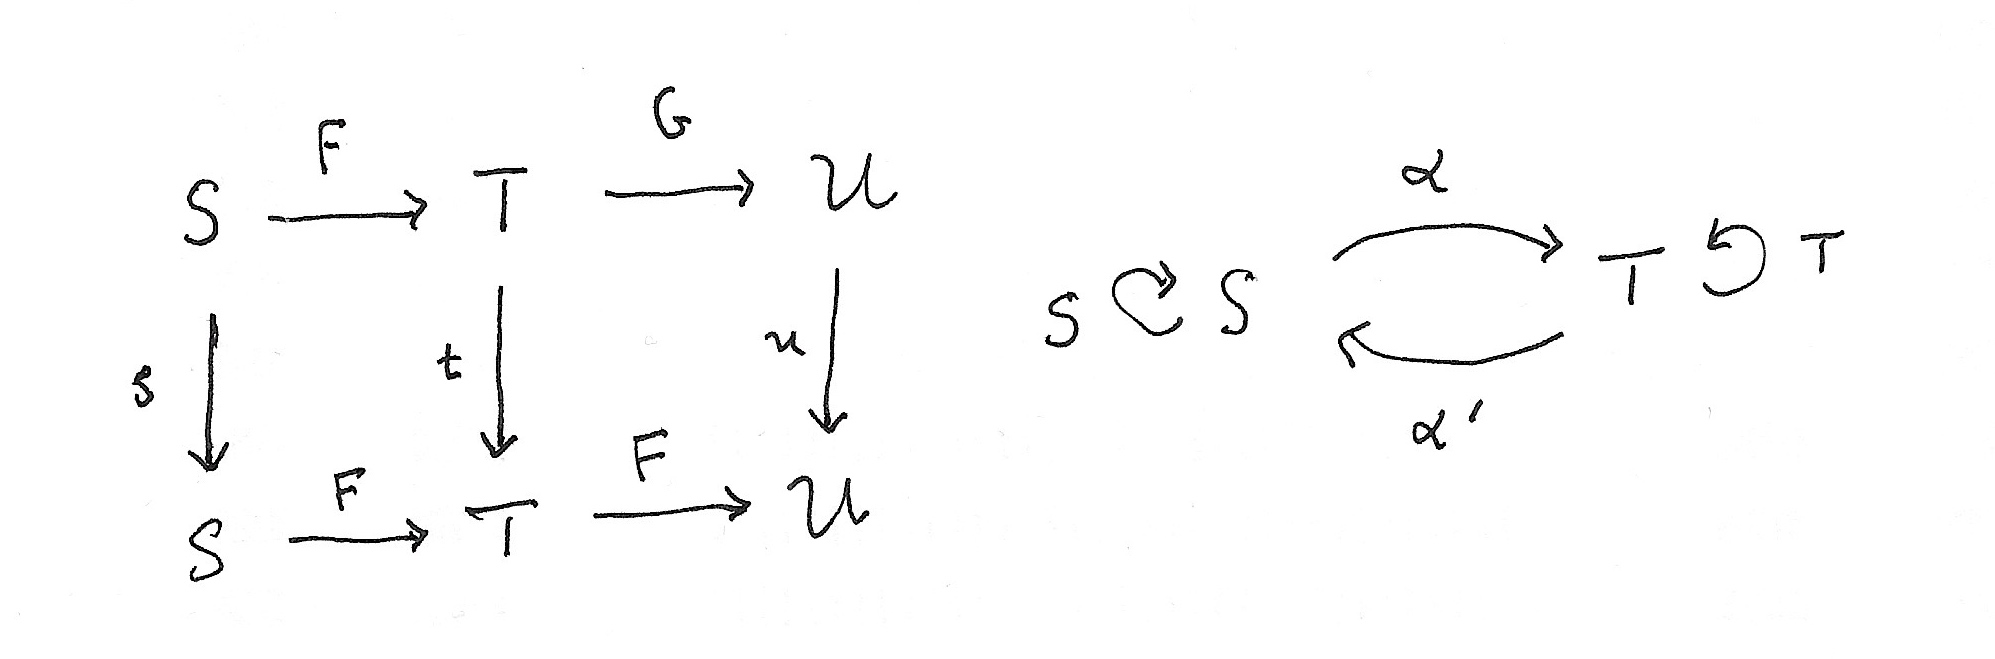
\includegraphics[width=0.7\textwidth]{Morphisms.png}
\caption{{\it The diagram on the left demonstrates that S${\overset F\longrightarrow}$T and T${\overset G\longrightarrow}$U implies $S{\overset {G\cdot F} \longrightarrow}$U, where space S has structure $s$, space T has structure $t$, and space U has structure $u$.  Spaces S and T are said to be isomorphic, if the diagram on the right commutes for some morphisms $\alpha$ and $\alpha'$.}}
\end{figure}

Figure 2 illustrates these definitions and demonstrates that composition of morphisms is associative.  If S${\overset F\longrightarrow}$T and T${\overset G\longrightarrow}$U, then S${\overset {G\cdot F} \longrightarrow}$U, where S, T and U are spaces (with structure).  Figure 2 also illustrates how 
definitions can be adopted from Category Theory.  For example, we say that spaces S and T are {\bf isomorphic} if the diagram of Figure 2(c) commutes for some morphisms $\alpha$ and $\alpha'$, denoted by S${\overset \alpha \cong}$T.  

Given S${\overset F\longrightarrow}$T, data F:X for any X is said to be in the {\it image} of F and data (S:X) is said to be in the {\it kernel} of F if (F:X)=(F:).  F may happen to be a space as well as a morphism.  In this case, the image of F is the same as the contents of F as a space.  
If F and G are morphisms from space S with structure $s$ to space T with structure $t$, we can define the {\it sum} of F and G by 
\begin{itemize}
\item[] F+G = $t\cdot$(F$\oplus$G)
\end{itemize}
Note the fact that F+G is a morphism relies on $t$ being a space, so that (F+G)$\cdot s$=$t\cdot$(F+G).  This addition is associative and is commutative 
if T is an algebraic space. If S and T are the same space, the composition F$\cdot$G is also a morphism since 
F$\cdot$G$\cdot$$s$=F$\cdot$$s$$\cdot$G=$s\cdot$F$\cdot$G, so the endomorphisms of a space form an algebraic structure.

\subsection{The Algebra of Endomorphisms}  

If $f$, $g$, and $h$ are endomorphisms of a space S with structure $s$, then $f\cdot(g\cdot h)=(f\cdot g)\cdot h$ is an associative 
multiplication and $f+(g+h)=(f+g)+h$ is an associative addition if we define $f+g = s\cdot(f\oplus g)$.  
Letting 1=S and 0=S$\cdot${\bf null}$\cdot$S, we have 
$1\cdot f=f\cdot 1=f$ and $0+f=f+0=f$.  Multiplication distributes over addition from the right $(f+g)\cdot h=(f\cdot h)+(g\cdot h)$.  

\begin{definition}
A {\bf semiring} is a collection of data with an associative multiplication with unit 1, with associative addition with unit 0, and where 
multiplication distributes over addition, from the right, as in $(f+g)\cdot h=(f\cdot h)+(g\cdot h)$.  
\end{definition} 

\noindent In summary, the endomorphisms of a space are a semiring with operations as described.  
If $f$, $g$, and $h$ are endomorphisms of S with structures $s$, we have the following.  
\begin{itemize}
\item[-]{If $f$ is a space as well as an endomorphism, $f\cdot(g+h)=f\cdot((f\cdot g)+(f\cdot h))$.  If 
$f$ is a distributive space then $f\cdot(g+h)=(f\cdot g)+(f\cdot h)$, so $f$ distributes from the left and the right.}
\item[-]{$0\cdot f=0$.  If $f$ is a space, $f\cdot 0=0$ also.  Since 1=S is always a space, $1\cdot 0=0$.  If 1=0, 
S=S$\cdot${\bf null}, so (S:X)=(S:) for all data X, in other words, S is a {\it constant} space.}
\item[-] {If $f$:X\ Y = $f$:Y\ X for all X,Y, $f$ is an {\bf algebraic} endomorphism.  If $f$ is algebraic, and $g$ is any endomorphism,  
$g\cdot f$ is algebraic.  If $f$ and $g$ are algebraic, so is $f+g$.  Thus, if Alg(S) are the algebraic endomorphisms, 
Alg(S) is a sub-semiring and is an ideal in the sense that $f\cdot$Alg(S)=Alg(S).}
\item[-] {Data (S:X) in S is {\bf in the kernel} of $f$ if (f:S:X) = (S:).  If $f$ is a space, then (S:X) and (S:Y) in the kernel of $f$ implies 
(S:X)\ (S:Y) is also in the kernel.  If the converse holds, we say that $f$ is a {\bf positive} space.  If $f$ and $g$ are positive, so is 
$f\cdot g$ and $f+g$ and 1 and 0, so positive endomorphism are a sub-semiring of mor(S).}
\item[-]{$f$ is an {\it involution} if $f\cdot f=1$.  Involutions $f$ and $g$ commute if and only if $f\cdot g$ is an involution.  If $f\cdot f=f$, $f$ is {\it idempotent}.}
\item[-]{If $f\cdot f'=f'\cdot f=1$ for some endomorphism $f'$, then $f$ and $f'$ are {\bf units} in the group of units.}
\item[-]{If $s$=S, then every endomorphism is a product $u\cdot i$ of a unit $u$ and an idempotent endomorphism $i$.} 
 \end{itemize}

\section{Examples}

\subsection{{\bf pass} and {\bf null}} 

    By definition, {\bf pass}:X=X and {\bf null}:X=() for any data X, so {\bf pass} and {\bf null} are both distributive, positive spaces.  As containers, {\bf pass} contains all data and {\bf null} contains only the empty sequence.  
Of the two, only {\bf null} is an {\it algebraic} space, and is ``more mathematical'' than {\bf pass}, which, after all, contains everything.  
From a preorder perspective, {\bf null}$\le$X$\le${\bf pass} for all X, {\bf pass} is only {\it compatible} with itself, and {\bf null} is {\it compatible} with every {\bf constant} space.  The kernel of {\bf pass} is the empty sequence only, while every data is in the kernel of {\bf null}.  {\bf pass} and {\bf null} are also 
{\it complementary} since they contain each other's kernels.  

\begin{figure}[h]
\centering
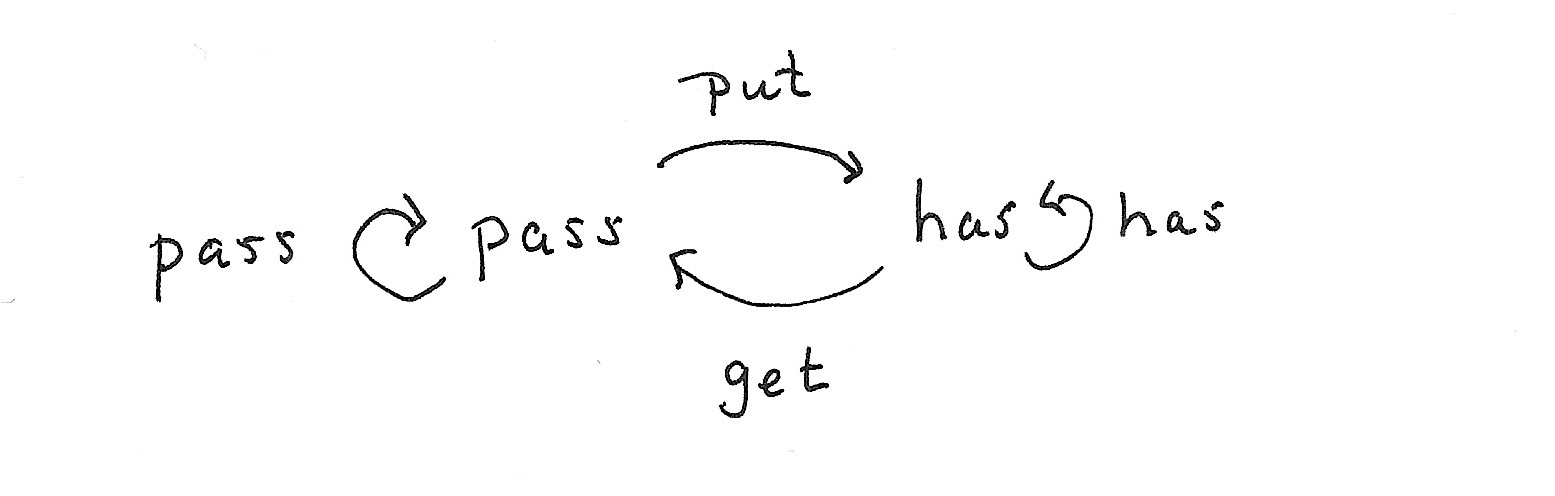
\includegraphics[width=0.6\textwidth]{Pass-has.png}
\caption{{\it In a definition adopted from Category Theory, if S with structure $s$ and T with structure $t$ are isomorphic, the top diagram commutes for some morphism $\alpha$ and some morphism $\alpha'$ where S and T function as their own `identity morphisms.' }}
\end{figure}

Since {\bf null}$\cdot f${\bf null}={\bf null}, {\bf null} is the only endomorphism of {\bf null}, so the semiring of {\bf null} contains only one data. 
On the other hand, the semiring of {\bf pass} includes all data with product $f\cdot g$ and with $f+g={\bf pass} \cdot (f \oplus g)$.  
Since {\bf pass}$\cdot f\cdot ${\bf pass}=$f$, any data $f$ is an endomorphism of {\bf pass}.  
Thus, every idempotent is an idempotent endomorphism of {\bf pass}, any space is a space endomorphism of {\bf pass}.  In a sense, {\bf pass} and {\bf null} are the simplest examples of spaces.  On the other hand a complete 
analysis of the semiring of {\bf pass} is far out of reach.  

\begin{figure}[h]
\centering
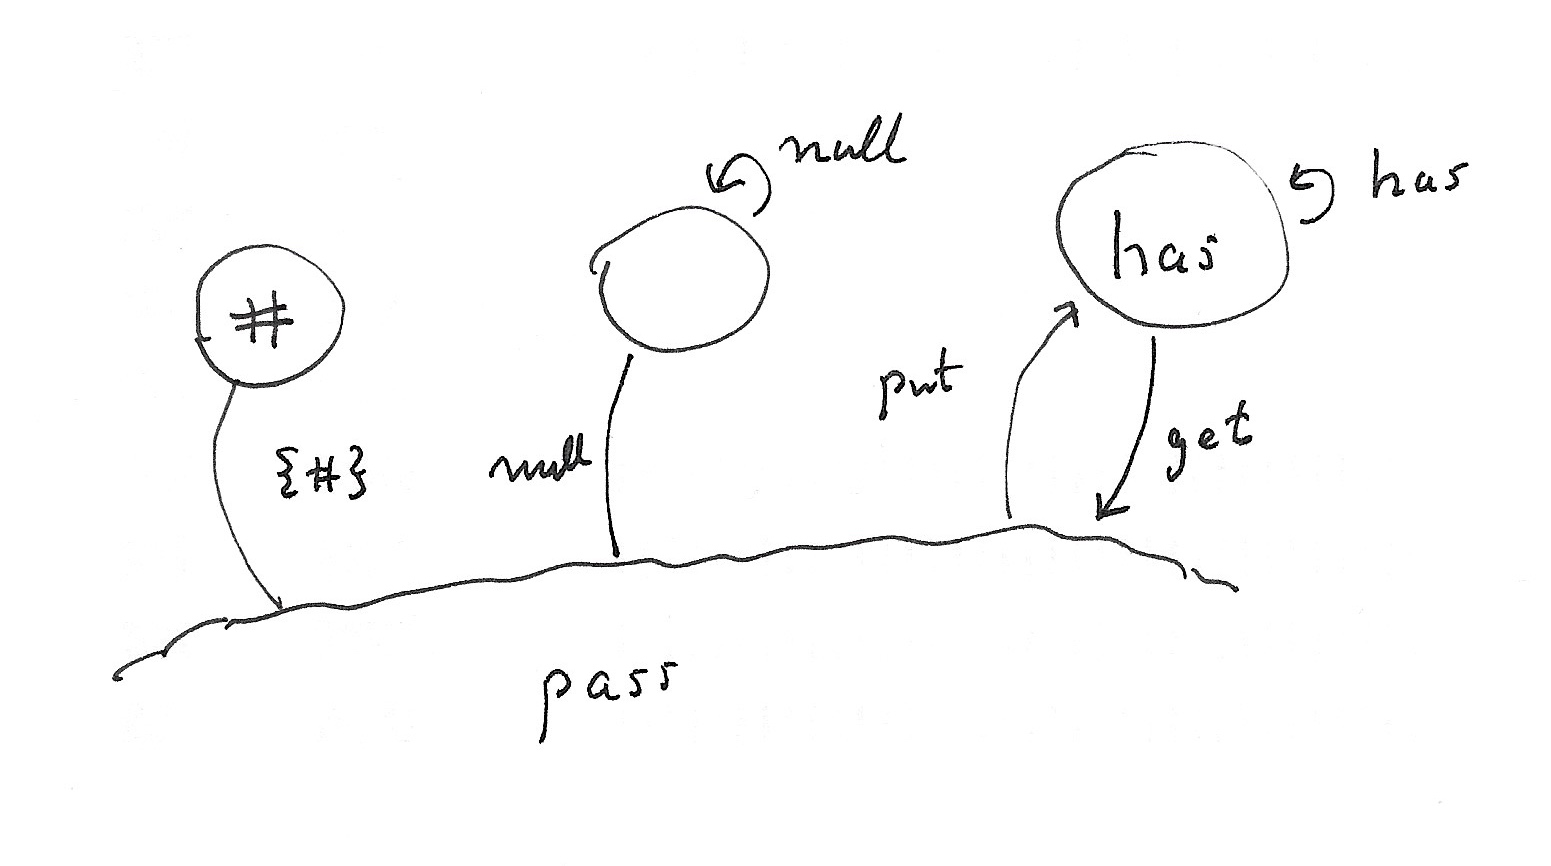
\includegraphics[width=0.6\textwidth]{Pass-garden.png}
\caption{{\it In a definition adopted from Category Theory, if S with structure $s$ and T with structure $t$ are isomorphic, the top diagram commutes for some morphism $\alpha$ and some morphism $\alpha'$ where S and T function as their own `identity morphisms.' }}
\end{figure}

As might be expected, {\bf pass} is isomorphic to subspaces of itself.  For example (Figure X), {\bf pass} is isomorphic to the space {\bf has} of (:X) atoms. 

\subsection{Natural Numbers}

Since concatenation is one of the two foundational operations, that suggests that the most ``organic'' version of natural numbers is to represent a natural number $n$ by a sequence of $n$ copies of some standard atom, for instance, if N is {\bf ap}\ \{$\vert$\}, N:X is a sequence of "sticks", one for each atom in X, and (N:X\ Y) is the natural number sum of the number of atoms 
in X plus the number of atoms in Y.  Since \{$\vert$\} is idempotent, N is a distributive space, and, therefore, a positive space with empty neutral data.  The kernel of N is also the empty 
sequence since only  
Without additional structure, the endomorphisms of N are data N$\cdot f\cdot$N for some data f, and this includes any function from naturals to naturals in the ordinary sense.  

    To add structure to N or to any space, one must find a space endomorphism of N, such as 
\begin{itemize}
\item[(a)]{N is a space endomorphism of itself.}
\item[(b)]{{\bf const}\ $\vert\ \vert\ \vert$, is a space endomorphism, since all constants are spaces.}
\item[(c)]{{\bf mod}\ $\vert\ \vert$, is a space endomorphism (mod $\vert\ \vert$:X is the number of atoms in X modulo 2)}
\item[(d)]{{\bf less}\ $\vert\ \vert\ \vert$, (min $\vert\ \vert\ \vert$:X is the minimum of 3 and the number of atoms in X)} 
\end{itemize}
where {\bf const} and {\bf less} happen to be pre-defined (see Glossary), and {\bf mod} has been defined via 
\begin{itemize}
\item{}def mod : \{while frontstrip A:B\} 
\end{itemize}
so, for instance, {\bf mod}\ $\vert\ \vert$:X repeatedly removes two vertical bars, if possible, stopping when the result no longer changes. 

\subsection{An isomorphism theorem}

\begin{fact}  If space $S{\overset \alpha \cong}T$ is an isomorphism of spaces, then the monoids of S and T are isomorphic.  
If $\alpha$ and it's inverse are distributive, the semirings of S and T are isomorphic as well. 
\end{fact}

As a consequence, $S$ and $T$ have the same involutions, idempotents, units, structure endomorphisms.  If $\alpha$ and it's inverse are distributive, then $S$ and $T$ also have the same spaces.  [Q?] If $S$ is algebraic, is $T$ also?  If $S$ is positive, is $T$ also?

\begin{figure}[h]
\centering
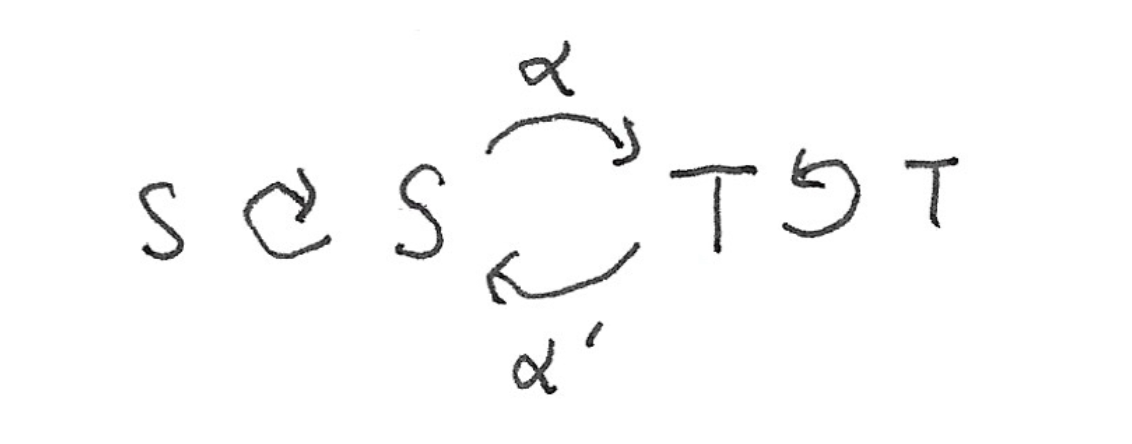
\includegraphics[width=0.6\textwidth]{isomorphism.png}
\caption{{\it In a definition adopted from Category Theory, if S with structure $s$ and T with structure $t$ are isomorphic, the top diagram commutes for some morphism $\alpha$ and some morphism $\alpha'$ where S and T function as their own `identity morphisms.' }}
\end{figure}

\section{Glossary}

For example, starting with context $\delta$, we can add more atoms of the form $\delta_a:c\mapsto c$:
\begin{enumerate}
\item[-]{$\delta_{(:)}$ : ((:) A : B) $\mapsto$ ((:) A : B), {\it single bit atoms where ((:):), ((:):(:)) are zero,one respectively.}}
\item[-]{$\delta_{((:):)}$ : (((:):) A : B) $\mapsto$ (((:):) A : B), {\it eight bit bytes.}}
\item[-]{$\delta_{((:):(:))}$ : (((:):(:)) A : B) $\mapsto$ (((:):(:)) A : B), {\it byte sequences}.}
\end{enumerate}
so that text strings or other data are atomic data within $\delta\cup\delta_{(:)}\cup\delta_{((:):)}\cup\delta_{((:):(:))}$.  We can then proceed to add named 
definitions that `get coda components':
\begin{enumerate}
\item[-]{$\delta_{\bf pass}$ : ({\bf pass} A:B) $\mapsto$ B}
\item[-]{$\delta_{\bf null}$ : ({\bf null} A:B) $\mapsto$ ()}
\item[-]{$\delta_{\bf right}$ : ({\bf right} A:B) $\mapsto$ B} 
\item[-]{$\delta_{\bf arg}$ : ({\bf arg} A:B) $\mapsto$ A} 
\end{enumerate}
and can add definitions for simple combinatorics 
\begin{enumerate}
\item[-]{$\delta_{\bf ap}$ : ({\bf ap} A : b B) $\mapsto$ (A:b) (ap A:B), {\it apply A to each atom in B.}}
\item[-]{$\delta_{\bf rev}$ : ({\bf rev} A : B b) $\mapsto$ b (rev : B), {\it reverse the order of atoms in B.}}
\end{enumerate}

definitions computing the boolean value of data 
\begin{enumerate}
\item[-]{$\delta_{\bf bool}$ : ({\bf bool} A : B b) $\mapsto$ () if B is empty, (:) if B is atomic, {\it logical value of B.}}
\end{enumerate}
definitions making new definitions  
\begin{enumerate}
\item[-]{$\delta_{\bf def}$ : ({\bf def} a : B) $\mapsto$ Add $\delta_a$ to context if $a$ is an unused invariant atom.} 
\end{enumerate}
As explained in reference \cite{PDF}, a language is introduced merely as one more definition where the domain of the language context $\delta_{\{\}}$ is 
codas starting with a curly brace as in (\{{\it language expression}\} A : B).  
\begin{enumerate}
\item[-]{$\delta_{\bf bool}$ : ({\bf bool} A : B b) $\mapsto$ () if B is empty, (:) if B is atomic, {\it logical value of B.}}
\end{enumerate}
definitions making new definitions  
\begin{enumerate}
\item[-]{$\delta_{\bf def}$ : ({\bf def} a : B) $\mapsto$ Add $\delta_a$ to context if $a$ is an unused invariant atom.} 
\end{enumerate}
As explained in reference \cite{PDF}, a language is introduced merely as one more definition where the domain of the language context $\delta_{\{\}}$ is 
codas starting with a curly brace as in (\{{\it language expression}\} A : B).  

%%%%%%%%%%%%%%%%%%%%%%%%%%%%%%%%%%%%%%%%%%%%%%%%%%%%%%%%%%%%%%%%%%%%%%%%
%%% \bibliography{jpsi}
\begin{thebibliography}{10}
\bibitem{PDF} {\it Pure Data Foundation of Mathematics and Computing}, Saul Youssef, 2023.
\bibitem{Berry} Nicholas Griffin (2003-06-23). {\it The Cambridge Companion to Bertrand Russell}. Cambridge University Press. p. 63. ISBN 978-0-521-63634-6.
\bibitem{Mazur} Barry Mazur, {\it When is one thing equal to some other thing?}, Harvard University, 2007,  {\rm https://people.math.harvard.edu/}$\sim${\rm mazur/preprints/when\_is\_one.pdf}. 
\end{thebibliography}
%%%%%%%%%%%%%%%%%%%%%%%%%%%%%%%%%%%%%%%%%%%%%%%%%%%%%%%%%%%%%%%%%%%%%%%%
\end{document}
